\subsection{Graph algorithms overview}
A number of data and network analytics questions on relational data can be posed as graph problems. For example, the transitivity or clustering coefficient tells us how clustered the nodes in a graph are. Clustered or small world networks having large value of clustering co-efficient have enhanced signal-propagation speed, synchronizability and computational power\cite{b1}. Nodes in sub-graphs with this property can be targetted for quick or low energy information disbursement. Another example involves finding the count and presence of certain structures in a graph. Identifying clusters of these patterns\cite{b2} or sub-graphs can indicate classes of predators in a food-web or interactions between sensors and effectors in a neural network\cite{b3}. A commonly occuring use case is of recommendations to connect with friends of friends in large social networks. It can be computed using the length of the path between two users\cite{b4}.
\subsection{Triangle counting as an application}
A k-truss is a maximal subgraph of a given graph such that each edge in it is contained in at least k-2 triangles. The k-truss in a graph is a sub-graph all the applications mentioned here can use. Triangles are the simplest subgraph in a graph. Counting the number of triangles in a graph is building block that can be used in finding the k-truss\cite{b5}. This makes triangle counting such a lucritive problem for the sub-graph isomorphism challenge\cite{b6}.
\subsection{Different approaches - set intersection/Linear algebra/map reduce/approximation methods for triangle counting}
Among the prominent methods for computing the count of triangles in a graph are ones using set intersection, linear algebra, map reduce and approximation methods. Set intersection algorithms \cite{b7} involve computing a set of all the possible edges that could generate triangles and counting the number of intersections with the original adjacency list. Innovations in the ordering of the members of the sets as well as ease of distribution of the work among multiple processes makes this class of algorithms highly performant\cite{b8} and ideal for implementation on shared memory systems. This class of algorithms is what inspired our work. Linear algebra approaches involve variantions of $\sum_{i,j}A^2\circ A$ where $A$ is the adjacency matrix\cite{b6}. One variantion involves splitting up the adjacency matrix into lower and upper triangular matrices not including the diagonal $A = L + U$. The product $B = L*U$ counts the number of paths of length 2 in the graph. Finding if the wedges close by performing a Hadamard product $C= A\circ B$ gives us the triangle count $\sum_{ij}(C)/2$\cite{b10, b9}. Map reduce approaches use frameworks such as Hadoop and distribute the adjacency lists among nodes arbitrarily. For a more detailed overview refer to \cite{b11,b12}. An interesting class of algorithms rely on wedge sampling to get an approximate count of the number of triangles. The work done in \cite{b13} shows an excellent use case that uses the birthday paradox to sample a set of wedges from the set of vertices and finding the approximate number of triangles by finding the number of closed wedges in this set.

\subsection{Challenges of parallelizing graph algorithms on modern architectures}
Graph algorithms are hard to parallelize and even harder to get good performance on modern architectures, both on many-core CPUs as well as on GPUs. The key challenge is that the nature of computations depends on the structure of the graph, i.e., the sparsity and specifically the sparsity pattern of the adjacency matrix of the graph. This means that the performance of the algorithm is directly dependent on the input graph's structure. This makes it very challenging to implement graph algorithms on parallel architectures where exclusive write access would be needed to obtain good parallel performance. At a more fundamental level, we also have to deal with having indirect memory access, due to the nature of adjacency lists, the most popular and efficient way to store graphs. Indirect memory access is bad for performance as it is difficult to utilize the cache effectively, leading to even higher costs for data access. One of the reasons for the popularity of linear algebra formulations for graph algorithms is the maturity of sparse linear algebra codes, especially on multicore CPU and GPUs. While these do indeed improve the performance to a certain extent, they are still sub-optimal. For one, unlike numerical algorithms, most graph algorithms, including triangle counting, are discrete in nature. Secondly, linear algebra formulations, especially those involving matrix-matrix products can require extensive data-movement and potentially increase both storage and compute requirements to $\mathcal{O}(n^2)$. For this reason, we wish to develop efficient graph algorithms that expose fine-grained parallelism and avoid indirect memory access. Such a formulation will enable efficient implementations on manycore processors and on GPUs. We now illustrate this idea using an example of set intersection, as that is one of the most expensive parts of triangle counting.

\subsection{Data-access concerns for set intersection}
Set intersection among two lists is an expensive operation if the lists are large. Consider the problem of finding the number of edges in a list $E'$, of length $m$,  that are also present in list $E$ of length $n$. A common approach for solving this problem is to sort $E$ with cost $\mathcal{O}(n\log n)$ and then perform $m$ binary searches for a total cost of $\mathcal{O}((m+n)\log n)$. In many cases this is reasonable. However, from a performance perspective, if $n$ is large, although the complexity of $\log n$ appears reasonable, it is very expensive on modern architectures, as this is random access into a very large array, each access potentially being retrieved from main-memory. An alternate approach is to sort both $E$ and $E'$, and performing a linear scan to determine matches. The complexity of this approach is similar at $\mathcal{O}(n\log n + m\log m)$, but this can be much faster, especially if using efficient sorting algorithms. This is in principle similar to using efficient linear algebra routines to obtain efficient implementations. However, it is possible to do even better if we design from first principles. We describe one such approach now.  

If we use a most significant bit radix sort to sort the lists $E$ and $E'$, we can improve the performance significantly, especially if we sort the lists simultaneously and use early termination. Note that a radix sort is efficient becuase data is accessed directly and in a streaming fashion, making it extremely amenable to deep cache hierarchies.   
Each element of the list is an ordered integer tuple $(u,v)$. For a value $(u,v)$ in $E$ to be equal to a value $(u',v')$ in $E'$, each bit in the binary representation of $u$ must match $u'$ and each bit in $v$ must match $v'$. We use this idea to bucket the entire list one bit at a time. Figure \ref{fig_radix_bucketing} gives an example of how a recursive bucket traversal can be used to perform intersection.

\begin{figure}
	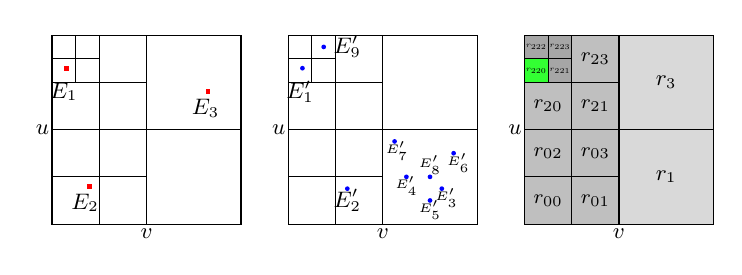
\begin{tikzpicture}[scale=0.3, every node/.style={scale=0.9}]
	% \draw[gray, very thin] (0,0) grid +(8,8);

	\begin{scope}[shift={(0,0)}]
	\draw (0,0) rectangle +(8,8);
	\draw[step=4] (0,0) grid +(8,8);
	\draw[step=2] (0,0) grid +(4,4);
	\draw[step=2] (0,4) grid +(4,4);
	\draw[step=1] (0,6) grid +(2,2);
    
	\fill[red!100] (0.5,6.5) rectangle +(0.2,0.2);
	\node at (0.5, 5.6) {\small $E_1$};
	\fill[red!100] (1.5,1.5) rectangle +(0.2,0.2);
	\node at (1.4, 0.9) {\small $E_2$};
	\fill[red!100] (6.5,5.5) rectangle +(0.2,0.2);
	\node at (6.5,4.9) {\small $E_3$};
	
	\node at (4,-0.4) {\small $v$};
	\node at (-0.4,4) {\small $u$};
	\end{scope}	 	
	
	\begin{scope}[shift={(10,0)}]
	\draw (0,0) rectangle +(8,8);
	\draw[step=4] (0,0) grid +(8,8);
	\draw[step=2] (0,0) grid +(4,4);
	\draw[step=2] (0,4) grid +(4,4);
	\draw[step=1] (0,6) grid +(2,2);
    
	\fill[blue!100] (0.6,6.6) circle (0.1);
	\node at (0.5, 5.6) {\small $E'_1$};
	\fill[blue!100] (2.5,1.5) circle (0.1);
	\node at (2.5, 1) {\small $E'_2$};
	\fill[blue!100] (6.5,1.5) circle (0.1);
	\node at (6.7, 1.1) {\tiny $E'_3$};
	\fill[blue!100] (5,2) circle (0.1);
	\node at (5, 1.6) {\tiny $E'_4$};
	\fill[blue!100] (6,1) circle (0.1);
	\node at (6, 0.6) {\tiny $E'_5$};
	\fill[blue!100] (7,3) circle (0.1);
	\node at (7.2, 2.6) {\tiny $E'_6$};
	\fill[blue!100] (4.5,3.5) circle (0.1);
	\node at (4.6, 3.1) {\tiny $E'_7$};
	\fill[blue!100] (6,2) circle (0.1);
	\node at (6, 2.5) {\tiny $E'_8$};
	\fill[blue!100] (1.5,7.5) circle (0.1);
	\node at (2.5, 7.5) {\small $E'_9$};
	
	\node at (4,-0.4) {\small $v$};
	\node at (-0.4,4) {\small $u$};
	\end{scope}

	\begin{scope}[shift={(20,0)}]
	\fill[gray!30] (0,0) rectangle +(8,8);
	\fill[gray!50] (0,0) rectangle +(4,4);
	\fill[gray!50] (0,4) rectangle +(4,4);
	\fill[gray!70] (1,6) rectangle +(1,1);
	\fill[gray!70] (1,7) rectangle +(1,1);
	\fill[gray!70] (0,7) rectangle +(1,1);
	\fill[green!80] (0,6) rectangle +(1,1);
	
	\draw (0,0) rectangle +(8,8);
	\draw[step=4] (0,0) grid +(8,8);
	\draw[step=2] (0,0) grid +(4,4);
	\draw[step=2] (0,4) grid +(4,4);
	\draw[step=1] (0,6) grid +(2,2);
	
	\node at (6,2) {\small $r_1$};
	\node at (6,6) {\small $r_3$};
	\node at (1,1) {\footnotesize $r_{00}$};
	\node at (3,1) {\footnotesize $r_{01}$};
	\node at (1,3) {\footnotesize $r_{02}$};
	\node at (3,3) {\footnotesize $r_{03}$};
	\node at (1,5) {\footnotesize $r_{20}$};
	\node at (3,5) {\footnotesize $r_{21}$};	
	\node at (3,7) {\footnotesize $r_{23}$};
	\node[scale=0.6] at (0.5,6.5) {\tiny $r_{220}$};
	\node[scale=0.6] at (1.5,6.5) {\tiny $r_{221}$};
	\node[scale=0.6] at (0.5,7.5) {\tiny $r_{222}$};
	\node[scale=0.6] at (1.5,7.5) {\tiny $r_{223}$};
	
	\node at (4,-0.4) {\small $v$};
	\node at (-0.4,4) {\small $u$};
	\end{scope}
	
	\end{tikzpicture}
\caption{\label{fig_radix_bucketing}From left to right: Elements of edge list $E$ with the bucket traversal overlay; elements of edge list $E'$ with the bucket traversal overlay; bucket traversal with region labels.}
\end{figure}

To perform bucketing, we first take the integer $u$ and mask the highest bit. The resultant value is concatenated with the masked highest bit of $v$. The resultant value is a number between 0 and 3. This lets us put each value in $E$ and $E'$ into the buckets $r_0$ through $r_3$ as shown in the last figure in figure \ref{fig_radix_bucketing}. From this point we will recursively compute intersections only if both $E$ and $E'$ have edges in the bucket. As shown in the first and second of figure \ref{fig_radix_bucketing} we can see that bucket $r_1$ in $E$ does not have any edges while bucket $r_3$ in $E'$ does not have any edges. Hence, we do not need to recurse in these buckets at all. Now $r_1$ has edges $E'_3$ through $E'_8$ which do not need to be tested. We have eliminated the need to test 6 out of 9 edges in $E'$. This is a significant reduction in work. Also, $r_3$ is eliminated as a potential bucket for recursion in $E$ removing the need to test edge $E_3$. In the next level of recursion we eliminate buckets $r_{00}$ through $r_{03}$ as well as $r_{20}, r_{21}, r_{23}$. Recursing on $r_{22}$ further we see that $r_{220}$ is the only bucket which has edges both in lists $E$ and $E'$. $E'_9$ in bucket $r_{223}$ does not have corresponding edges in $E$. Since $r_{220}$ has very few elements in both $E$ and $E'$ we can compare each element in $E'$ to each element in $E$ for $r_{220}$ to find that $E'_1$ has a matching edge $E_1$ and is the only edge also present in list $E$.
Although this is a synthetic example, it demonstrates that sparse distributions on $E$ and $E'$ will result in elimination of a large set of candidates for intersection quickly. Each level of recursion is $O(|E|+|E'|)$ i.e. it is $O(n)$ in the size of the lists.

% \section{Background and Related work}
% \subsection{Parallel Graph algorithms}
% \subsection{GPU}
% \subsection{Linear algebra}
% \subsection{Graph}
% \subsection{Triangle counting}